% !TeX spellcheck = en_GB
\documentclass[10pt,a4paper]{article}
\usepackage[latin1]{inputenc}
\usepackage{amsmath}
\usepackage{amsfonts}
\usepackage{amssymb}
\usepackage{graphicx}
\graphicspath{{../../Figures/}{./figures/}}

\usepackage{todonotes}
\usepackage{longtable}
\usepackage{chngpage}
\usepackage{booktabs}
\usepackage[
backend=biber,
natbib=true,
style=authoryear,
sorting=none]{biblatex}
\addbibresource{PAP15.bib}
\usepackage{hyperref}
\usepackage[caption=false,font=footnotesize]{subfig}


\title{PAP Report 2015\\
\large 
An Investigation into Trust and Reputation Frameworks for \\
Collaborative Teams of Autonomous Underwater Vehicles }

\author{Andrew Bolster, \\
		\large Supervised by \\
		Prof. Alan Marshall and Prof. Simon Maskell}
\date{May 19, 2015}


\begin{document}
\maketitle
\section{Overview}
\begin{itemize}
	\item \textbf{Started:} October 2011 @ Queen's University Belfast
	\item \textbf{Transferred:} October 2013 @ University of Liverpool
	\item \textbf{Target Submission:} November 2015
\end{itemize}
	
The project is focused developing a multi-vector trust management framework (TMF) for collaborative operation of autonomous systems.
	
Specifically, this project is looking at the relationships between physical behaviour and communications behaviour within teams of autonomous underwater vehicles (AUVs) for uses related to mine counter measures and port protection for defence, as well as persistent survey behaviour for environmental and petrochemical applications.
	
This work is undertaken as part of The UK-France joint PhD Programme which is jointly managed by Direction G�n�rale de l'Armement (DGA) and Defence Science and Technology Laboratory. It was agreed at the 2010 Anglo-French Summit as one of the ten priorities in 2011 for the Anglo French Defence Research Group (AFDRG).
In 2011, five PhDs were funded (two from the UK and three from France), In 2012, the programme grew to nine PhDs (five from the UK and four from France). In 2013 a further ten PhDs were funded (five from the UK and five from France). These PhDs are currently investigating a variety of topics including meta-materials, synthetic biology, sensors, vehicle armour, and human and social sciences as well as this project's work in autonomous underwater vehicles.
	
\section{Summary of Current Outputs}
Since the launch of the project, the majority of time has been spent developing a bespoke simulation framework based on Python, developing a variety of ``normal'', ``abnormal'' and ``malicious'' physical behaviours, as well as developing a range of analytical techniques to detect and identify these behaviours to an extremely high degree of statistical accuracy, i.e.in a Monte Carlo style random repeat experiment, the classifier is correct and confident a significant percentage of experimental runs.
	
Major outputs and research interactions of the project are: 
\begin{itemize}
	\item Attendance at UComms 2012 (Sestri Levante, Italy)
	\item Poster Presentations in 2012 (Kassam, Oxford) and 2013 (Heathrow, London)
	\item Summer Research Placement with DSTL (Software Systems and Dependability for Autonomous Teams)(2013, Portsdown West, Portsmouth)
	\item Short Paper Presentation to the Association for the Advancement of Artificial Intelligence (AAAI) on ``A Multi Vector Trust Framework for Autonomous Systems'' (2014, Stanford, CA)\cite{Bolster2014}
	\item Technical Report for the UK/US/CAN/AUS/NZ Technical Cooperation Programme ((2014). Analysis of Trust Interfaces in Autonomous and Semi-Autonomous Collaborative MHPC Operations. The Technical Cooperation Program, Technical Report TR-C3I-06-2014) (June 13 - April 14)\cite{Bolster2014a}
	\item DSTL CDE Collaboration with NPL and Plextek Ltd. on ``Precision Timing and Navigation, Challenge 1: Resilient Time and Location Estimation for Networked Assets'' (CDE 33135) (Oct 13-May 14)
	\item Rejected submission to AdHocNow15 
	\item ``Single and Multi-Metric Trust Management Frameworks for use in Underwater Autonomous Networks'' submitted to TrustCom15 (Pending)
\end{itemize}
	
\section{Field Background}
\subsection{What is 'Trust'?}
``Trust'' is a word that gets used a lot in many different ways. Mirriam Webster's Dictionary defines trust as ``assured reliance on the character, ability, strength, or truth of someone or something''.
	
This rather far reaching definition is very attractive to distributed network design as this ``trustworthiness''  can be used to inform autonomous actors, or nodes, to the ``best'' courses and paths to action, making them more efficient and resilient in their operation.
Within this context, we define trust as ``The Expectation of an actor performing a certain task or range of tasks within a certain confidence or probability''. 
	
In the real world use-case of deployable autonomous systems for survey or other application, this trust can take on two real forms;
\begin{itemize}
	\item Design Trust, where there is an expectation that a system of systems will perform as specified or designed in operation, and
	\item Operational Trust, that is that the individual systems within a larger system will and are performing as designed in the field. It is this area with which we are particularly concerned.
\end{itemize}
	
\subsection{Trust Management Frameworks (TMFs)}
	
This desire for operational trust in mobile ad-hoc networks has lead to the development of several Trust Management Frameworks (TMFs), where such frameworks provide information regarding the estimated future states and operations of nodes within such a network. 
As such, the operation of such frameworks has been summarised as ``collecting the information necessary to establish a trust relationship and dynamically monitoring and adjusting the existing trust relationship'' \cite{Li2007}.
	
Almost all of the work currently applied to establishing trust in mobile ad-hoc networks (MANETs) relies either on shared key exchanges with a centralised trust repository (PKI) or with exclusive assessment based on communications behaviour alone, and in that case the vast majority only measure one value (eg packet forward likelihood). 
Within MANETs, the requirement for distributed trust comes from the decentralised and dynamic communication paths used; if a node moves or an environment changes, the network topology can completely change with paths containing potentially malicious nodes that can disrupt, modify, or reject communications coming from or going to a given node. 
The motivation for that application of TMFs to MANETs is that by taking historical performance information into accounts, malicious or inefficient actors can be at least detected and routed isolated, preventing further compromise to the distributed network.
	
These single metric TMFs provide malicious actors with a significant advantage if their activity is undetectable by that one assessed metric, especially if the attacker knows the metric in advance. The objective of operating a TMF is to increase the confidence in, and efficiency of, a system by reducing the amount of undetectable negative operations an attacker can perform.
This space of potential attacks can be described as the ``Threat Surface''. In the case where the attacker can subvert the TMF, the metric under assessment by that TMF does not cover the threat mounted by the attacker. In turn, this causes a super-linearly negative effect in the efficiency of the network. 
	
The TMF is assumed to have reduced the threat surface when in fact it has simply made it more advantageous to attack a different part of it.
\cite{Huang2010a} also raised the need for a more expanded view of trust but did so with a domain-partitioning approach rather than combining trust assessments from multiple domains within networks. 
	
\subsection{Multi-Parametric Trust Management Frameworks}
Guo developed a form of vectorised trust that allowed the combination and cross-correlation of a range of communications observations (Packet error rate, Noise characteristics, Delay, Throughput, etc) not only as a combined singular value in the form of a Grey Interval, but also presented the ability to use this vectorised trust assessment to not just detect but also identify malicious or abnormal behaviours through weight assessment perturbations \cite{Guo11}.
	
\begin{figure}[h!]
	\missingfigure{Bellas Graphs demonstrating weighted delta}
	\caption{Example of weight-based attack classification taken from (Guo, Marshall \& Zhou 2011)}
\end{figure}

Guo\cite{Guo11} demonstrated the ability of Grey Relational Analysis (GRA)\cite{Zuo1995} to normalise and combine disparate traits of a communications link such as instantaneous throughput, received signal strength, etc. into a Grey Relational Coefficient, or a ``trust vector''.

In the case of the terrestrial communications network used in \cite{Guo11}, the observed metric set $X = {x_1,\dots,x_M}$ representing the measurements taken by each node of its neighbours at least interval, is defined as $X=[$packet loss rate, signal strength, data rate, delay, throughput$]$.
The trust vector is given as
%
\begin{align}
\label{eq:grc}
\theta_{k,j}^t = \frac{\min_k|a_{k,j}^t - g_j^t| + \rho \max_k|a_{k,j}^t-g_j^t|}{|a_{k,j}^t-g_j^t| + \rho \max_k|a_{k,j}^t-g_j^t|} \\
\phi_{k,j}^t = \frac{\min_k|a_{k,j}^t - b_j^t| + \rho \max_k|a_{k,j}^t-b_j^t|}{|a_{k,j}^t-b_j^t| + \rho \max_k|a_{k,j}^t-b_j^t|} \notag 
\end{align}
%
where $a_{k,j}^t$ is the value of a observed metric $x_j$ for a given node $k$ at time $t$, $\rho$ is a distinguishing coefficient set to $0.5$, $g$ and $b$ are respectively the '``good'' and ``bad'' reference metric sequences from $\{a_{k,j}^t k=1,2\dots K\}$, e.g. $g_j=\max_k({a_{k,j}^t})$,  $b_j=\min_k({a_{k,j}^t})$ (where each metric is selected to be monotonically positive for trust assessment, e.g. higher throughput is always better). 
	
For applications involving low fidelity, temporally sparse metrics with unknown statistical distributions, this Grey Relational Analysis is a more stable comparative analysis, providing an interval of potential trust values rather than fuzzy-logic or the Bayesian-Beta distributions found in current TMFs \cite{Liu2006}.

However, this still ignores the usefulness of physical behaviours in the development of trust assessments, which became the basis for this project.

\section{Project Objectives and Novelty}

The aims of this project are to extend this ``vectorised'' methodology to not only combine individual trust metrics (observations) into trust vectors, but to combine such vectorised assessments of trust across ``domains'' (i.e. combining trust assessments based on observations in the communications domain with trust assessments based on observations in the physical domain).

In single metric trust, such as the use of packet loss rate in other TMFs, this only detects a relatively small area of the potential attack space.
Combining several domain specific metrics, in this case in communication, provides not only the capability to detect a much wider range of attack types, but also to discriminate between them, potentially disclosing of the tactics of an attacker.

Our hope is that by using multiple domains together, we can provide a higher level, strategic point of view on an attacker or attackers, enabling the generation of preventative and reactive strategies to defend against them. This would leave even the most knowledgeable attacker with no option but to behave properly to avoid detections, eliminating any potential reward they could achieve without detection.

\begin{figure}[h!]
	\missingfigure{Bellas Graphs demonstrating weighted delta}
	\caption{With the addition of further metrics, the threat surface available to an attacker is greatly reduced}
\end{figure}

Our main goal in this project has been to investigate if the methodologies that Guo applied to communications, can equally be applied to physical behaviour. 
Our approach to this has been to develop an agent based simulation platform built in Python, emulating both the physical and communicative environments for teams of flocking nodes performing some task, such as mine counter measure survey, port protection, mother-ship protection and others.

This interaction in the physical world opens up a range of metrics that can be used for trust assessment, in an effort to further restrict undetected malicious behaviour on the exposed threat surface of a network.

In summary, the novelties of the work accomplished so far are:
\begin{itemize}
	\item Fused Trust Assessment using Physical Behaviour in collaborative mobile autonomous networks (CMAN)
	\item Analytical comparison of Marine and Terrestrial Communicative trust environments
	\item Exploration and Demonstration of the advantages of multiple metric trust over single metric trust (in communications)
	\item Defined protocol for quantitative assessment of Metric suitability through comparative regression analysis
\end{itemize}

Novelties remaining to be produced prior to submission:
\begin{itemize}
	\item Definition of asynchronous trust assessment with back-propogation (required to deal with both multi-domain and time delay factors in reporting)
	\item Demonstration of advantage between single domain (MTFM) and multi domain trust.
\end{itemize}

\section{Current Progress and Results}

\subsection{Physical Behaviours}

Through collaboration NATO's Centre for Maritime Research and Experimentation based in Italy, and the UK's Defence Science and Technology Laboratory, we settled on a range of observable metrics based on the position and attitudes of other nodes in the group.
These were;
\begin{itemize}
	\item The Inter Node Heading Deviation (INHD), i.e. the deviation in heading from a local group average,
	\item The Inter Node Distance Deviation (INDD), i.e. the deviation of a given node's position with respect to the average node spacing across the rest of the local group,
	\item And The Node's Absolute Speed.
\end{itemize}

Along with metric selection, we also arrived at a few sample 'Misbehaviours' covering both malicious and non-malicious non-optimal behaviours which were simulated in the framework. These were:
\begin{itemize}
	\item \textbf{The Shadow}, where a node is following the fleet without appropriate mission knowledge such as the waypoints in a patrol path, modeling an 'infected' or masquerading node in the fleet
	\item \textbf{The Spy}, where a node consistently or intermittently rises to the top of the fleet, potentially surfacing to relay mission information to an unauthorised third party via a back-channel communications channel such as RF
	\item \textbf{The Sloth}, where a node is selfishly conserving energy by not making complete patrol paths or consistently taking a minimal path around the tolerances of the waypoint path
	\item \textbf{The Stalker}, where a node in a multi-node system preferentially 'tails' a given node above others
	\item \textbf{The Scoundrel}, where a node falsely reports it's position or velocity with the intention to corrupt any collaborative positioning system
	\item \textbf{The Slow Coach}, where a node is operating correctly but has a defect in it's power train causing reduced maneuverability, i.e. a runtime defect in an otherwise good node
	\item \textbf{The Spin Doctor}, likewise is operating correctly but it's Inertial Navigation System is damaged and consistently bears left/right by some level.
\end{itemize}

Initially we've only directly considered Shadow and Slow Coach behaviours, as this presents a useful side effect of trust based on physical behaviour; the ability for a network to self-test it's health by discerning the difference between broken and malicious behaviour.

In a simple port protection scenario, where nodes are patrolling around a series of waypoints around an area, We can demonstrate this detective and selective power through a series of  graphs that clearly justify the abstraction of such metrics into a trust value.

\begin{figure}[h!]
	\missingfigure{Behaviour Deviation Trust Curves}
	\caption{Charts showing deviation activation curves for three different simulated behaviours, with a fuzed trust value in the bottom row.}
\end{figure}


Each vertical of this chart shows a different behaviour; with the baseline waypointing behaviour in the middle, flanked on the left by the malicious ``Shadow'' behaviour and on the right by the benign but sub-optimal ``Slowcoach'' behaviour. The per-node metrics as described are shown in the horizontal, with Internode Heading Deviation at the top, followed by Absolute Speed and Distance Deviation in the middle and finally a combined trust 'vectorised' (dis)trust assessment in the bottom, based on a decaying windowed average of instantaneous trust assessments across observation types.

With this chart it's shown that the Slowcoach behaviour manifests itself in the Speed metric. more so than the Shadow behaviour. Using this information we can build a trust weight vector to discriminate between these two ostensibly similar behaviours.

With our current analysis we can do so with an average 96\% positive identification rate with a 1\% false positive rate, i.e.  instances where a Slowcoach is confidently detected as a Shadow and visa versa. (It should be noted that in this analysis, there were no cases where the malicious behaviour (Shadow) was misdetected as the purely abnormal/faulty behaviour (Slow Coach).

\subsection{Communications Behaviours}

The major amount of recent work has been concerned with the development and testing of simulated acoustic communications channels. Supposedly feature-complete implementations such as \cite{Miquel2008} were found to be incomplete and not totally tested, and this put back development by several months. 

However, we were able to incorporate our experiences under the DSTL/NPL/Plextek collaboration project (CDE 33135) to reimplement and improve both the routing and physical modelling used in the AUVNetSim framework. These implementations were validated against \cite{Stojanovic2007} and \cite{Stefanov2011}.

Then, having implemented Multi-parameter Trust Framework for MANETS (MTFM)\cite{Guo11}, Hermes\cite{Zouridaki2009}, and Optimal Trust Management Framework(OTMF)\cite{Li2008}, exploratory simulations were run to establish a comparable operation range for the simulated marine context.

\begin{table}[h]
	\caption{Comparison of system model constraints as applied between Terrestrial and Marine communications} \label{tab:sysconstraints}
	\begin{center}
		\setlength{\tabcolsep}{8pt}
		\begin{tabular}{lccc}
			\toprule
			Parameter & Unit & Terrestrial & Marine \\
			\midrule
			Simulated Duration & $s$ & 300 & 18000\\
			Trust Sampling Period & $s$ & 1 & 600 \\
			Simulated Area & $km^2$ & 0.7 & 0.7-4 \\
			Transmission Range & $km$ & 0.25 & 1.5 \\
			Physical Layer & & RF(802.11) & Acoustic\\
			Propagation Speed& $m/s$ & $3\times10^8$ & 1490\\
			Center Frequency& $Hz$ & $2.6\times10^9$ & $2 \times 10^4$ \\
			Bandwidth& $Hz$ & $22\times10^6$ & $1\times10^4$\\
			MAC Type & & CSMA/DCF & CSMA/CA\\
			Routing Protocol & & DSDV & FBR \\
			Max Speed & $ms^{-1}$ & 5 & 1.5 \\
			Max Data Rate & $bps$ & $5\times10^6$ & $\approx 240$ \\
			Packet Size & bits & 4096 &  9600 \\
			Single Transmission Duration & $s$ & 10 & 32 \\
			Single Transmission Size & bits & $10^7$ & $9600$ \\
			\bottomrule
		\end{tabular}
		\setlength{\tabcolsep}{6pt}
	\end{center}
\end{table}

Given the differences in delay and propagation between RF and marine networks, it would not be expected that the same application rates (e.g. packet emission rates or throughput) and node separations are equally stable in this environment.

\begin{figure}[h!]
	\missingfigure{Surface / 3D Plots of performance space for PER / Node Sep}
	\caption{Surface Plot showing performance gradient across varying packet emission rates and node separations}
\end{figure}

As the separation is increased, the emission rate at which the network becomes saturated decreases, reducing overall throughput. 
This throughput degradation is tightly coupled with the mobility, as increasing mobility leads to increasing delays as routes are constantly broken, re-advertised and re-established. 
For instance, where all nodes are static, we do not see significant drops in saturation rates until node separation approaches 800m, nearly double the initial estimate. 
When all nodes are randomly walking the saturation point collapses from 0.025pps at 300m to 0.015pps at 400m.
Our results indicate that the best area to continue operating in for a range of node separations is at 0.015pps, and that a reasonable position scaling is from 100m to 300m, beyond which communication becomes increasingly unstable, especially in terms of end-to-end delay.
These results are similar to work performed in \cite{Miquel2008}, and are expected in such a sparse, noisy, and contentious environment. 

Guo et al. introduced a range of misbehaviours, including modification of the packet loss rate of routing nodes and limiting throughput on a per-link basis as well as a selection of combined misbehaviours. 

Given that the established links are already heavily constrained, attacks such as introducing selective packet dropping or artificially adding to the already extreme and hugely variable delays would severely impact the general performance of the network beyond the scope of simple selfishness.
These direct malicious behaviours effectively trigger saturation collapses in operating regions of the network that should be stable.

Therefore, we select two more subtle misbehaviours to investigate; 
\begin{enumerate}
	\item Malicious Power Control (MPC), where $n_1$ increases its transmit and forwarding power by 20\% for all nodes \emph{except} communications from $n_0$ in order to make $n_0$ appear to be selfishly conserving energy to the rest of the team, while $n_1$ itself appears to be performing very well.
	\item Selfish Target Selection (STS), where $n_1$ preferentially communicates, forwards and advertises to nodes that are physically close to it in effort to reduce its own power consumption.
\end{enumerate}

\begin{figure}[h]
	\subfloat[Delay]{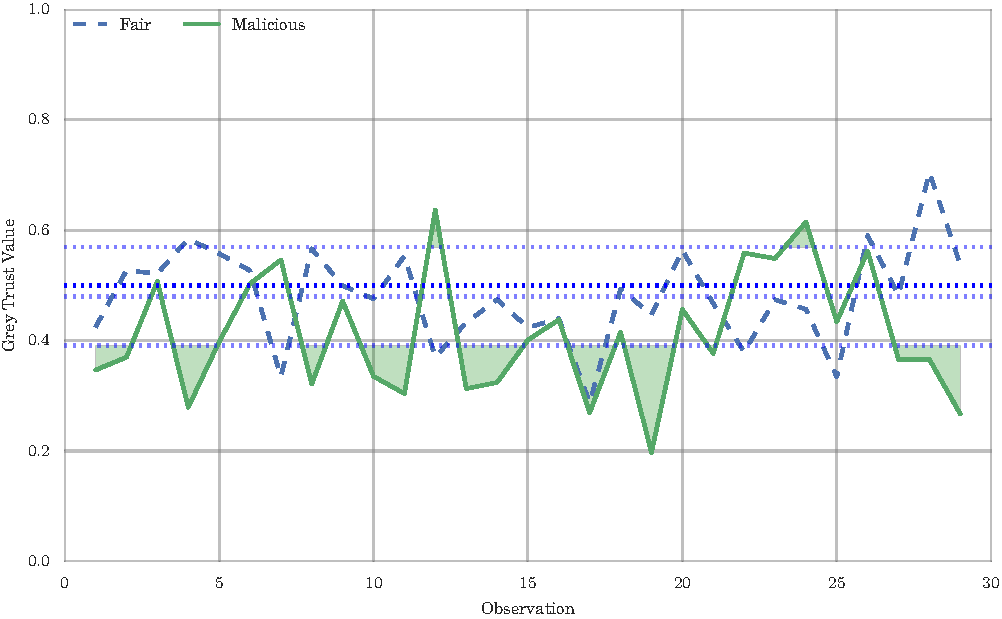
\includegraphics[width=.5\linewidth]{trust_bella_all_mobile_emph_ADelay_BadMouthingPowerControl} \label{fig:all_mobile_selfish_delay}}
	\subfloat[PLR]{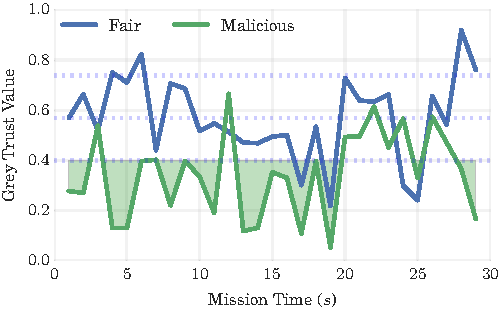
\includegraphics[width=.5\linewidth]{trust_bella_all_mobile_emph_PLR_BadMouthingPowerControl}\label{fig:all_mobile_selfish_plr}}
	\newline
	\subfloat[RX Power]{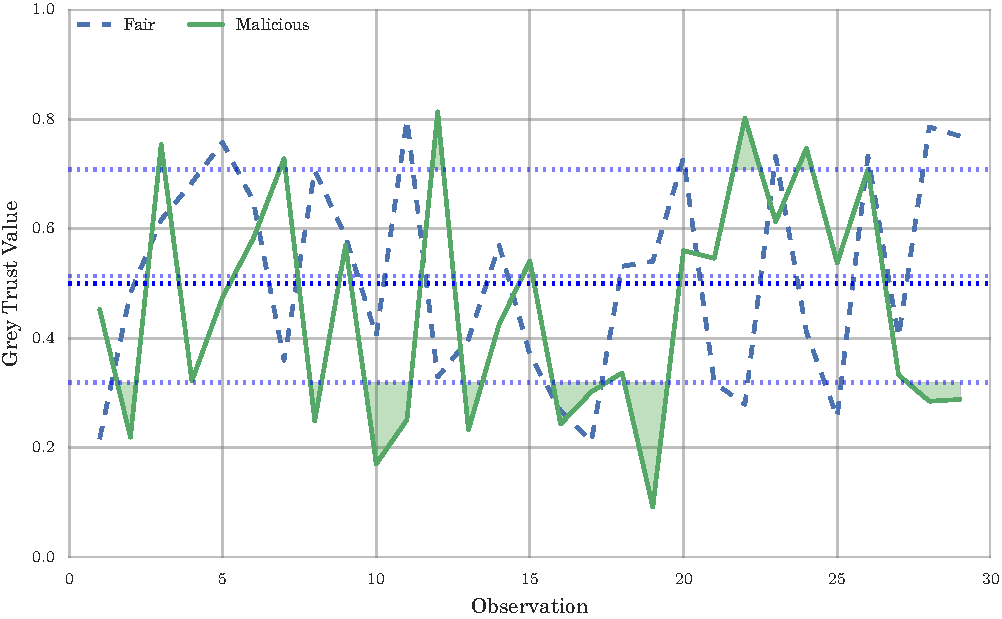
\includegraphics[width=.5\linewidth]{trust_bella_all_mobile_emph_ARXP_BadMouthingPowerControl} \label{fig:all_mobile_selfish_rxp}}
	\subfloat[TX Power]{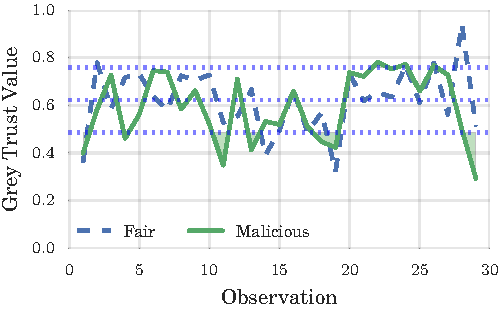
\includegraphics[width=.5\linewidth]{trust_bella_all_mobile_emph_ATXP_BadMouthingPowerControl}\label{fig:all_mobile_selfish_txp}}
	\newline
	\subfloat[RX Throughput]{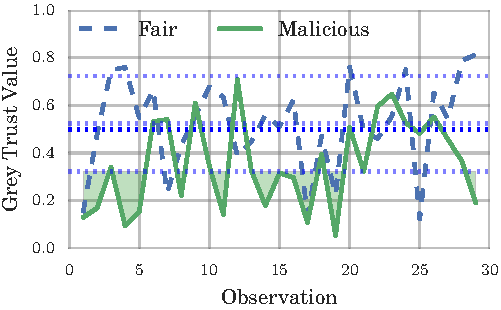
\includegraphics[width=.5\linewidth]{trust_bella_all_mobile_emph_RXThroughput_BadMouthingPowerControl} \label{fig:all_mobile_selfish_rxthroughput}}
	\subfloat[TX Throughput]{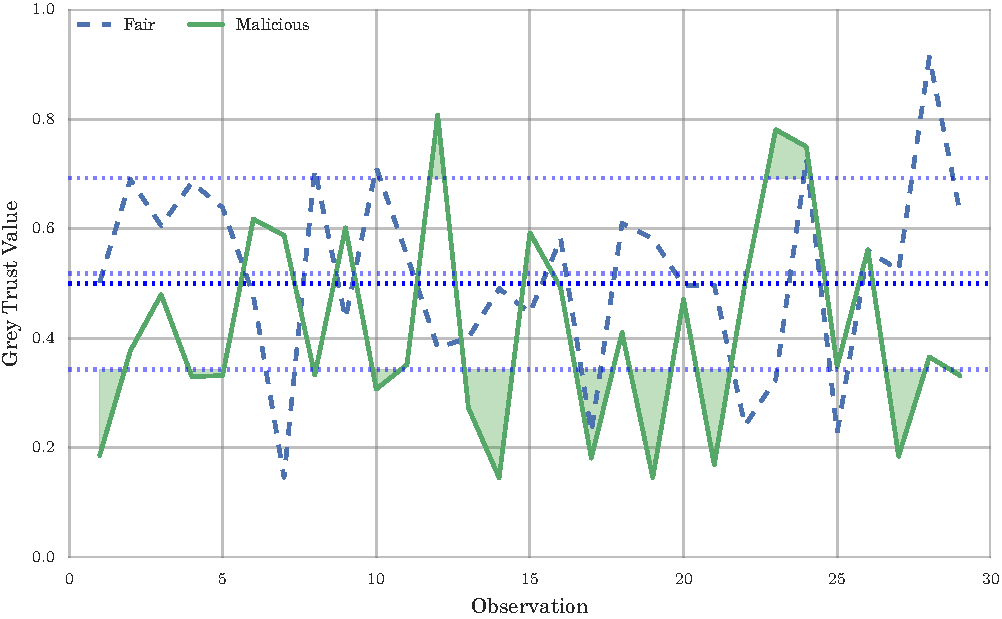
\includegraphics[width=.5\linewidth]{trust_bella_all_mobile_emph_TXThroughput_BadMouthingPowerControl} \label{fig:all_mobile_selfish_txthroughput}}
	\caption{$T_{1,MTFM}$ in the All Mobile case for the MPC behaviour, including dashed $\pm\sigma$ envelope about the fair scenario}
	\label{fig:all_mobile_selfish}
\end{figure}

\begin{figure}[h]
	\subfloat[Delay]{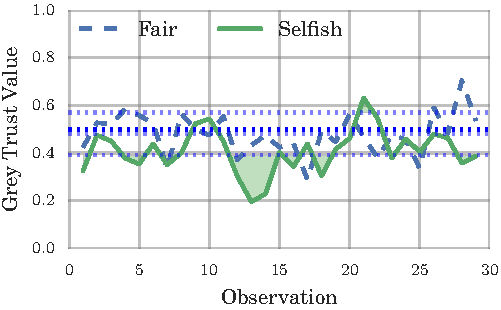
\includegraphics[width=.5\linewidth]{trust_bella_all_mobile_emph_ADelay_SelfishTargetSelection} \label{fig:all_mobile_selfish_delay}}
	\subfloat[PLR]{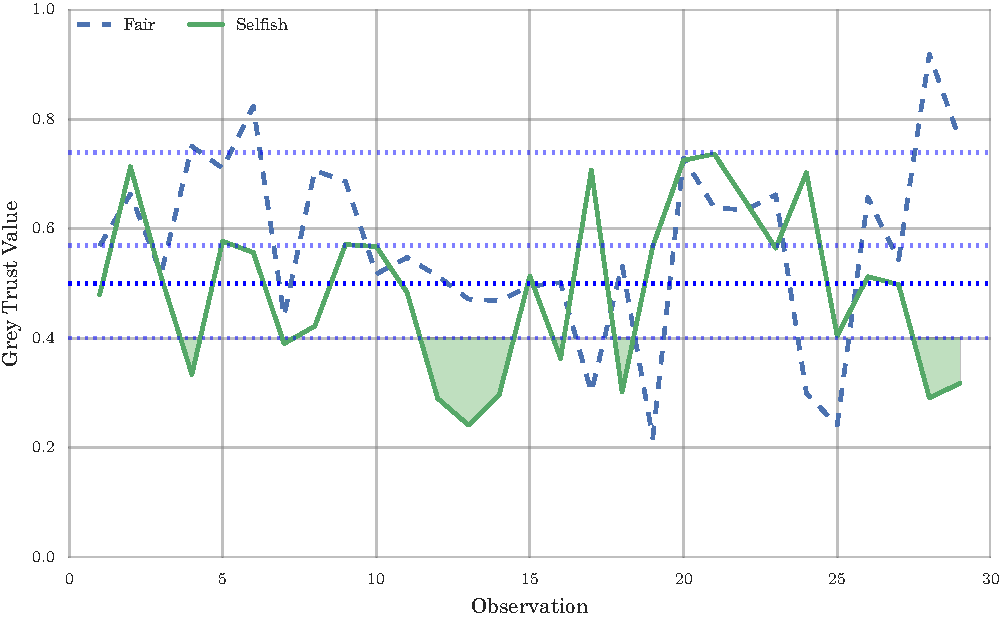
\includegraphics[width=.5\linewidth]{trust_bella_all_mobile_emph_PLR_SelfishTargetSelection}\label{fig:all_mobile_selfish_plr}}
	\newline
	\subfloat[RX Power]{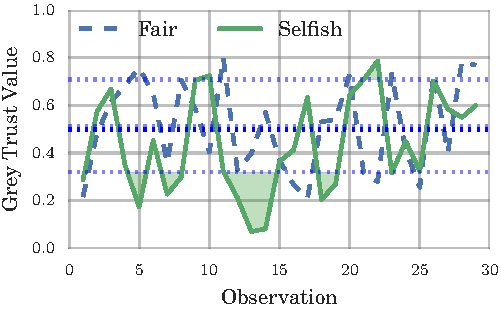
\includegraphics[width=.5\linewidth]{trust_bella_all_mobile_emph_ARXP_SelfishTargetSelection} \label{fig:all_mobile_selfish_rxp}}
	\subfloat[TX Power]{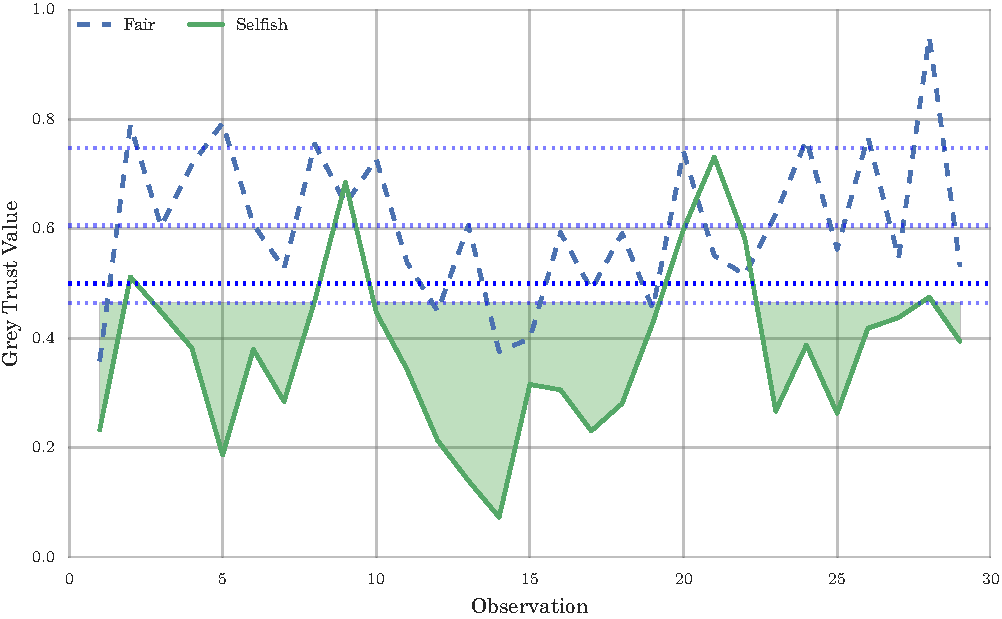
\includegraphics[width=.5\linewidth]{trust_bella_all_mobile_emph_ATXP_SelfishTargetSelection}\label{fig:all_mobile_selfish_txp}}
	\newline
	\subfloat[RX Throughput]{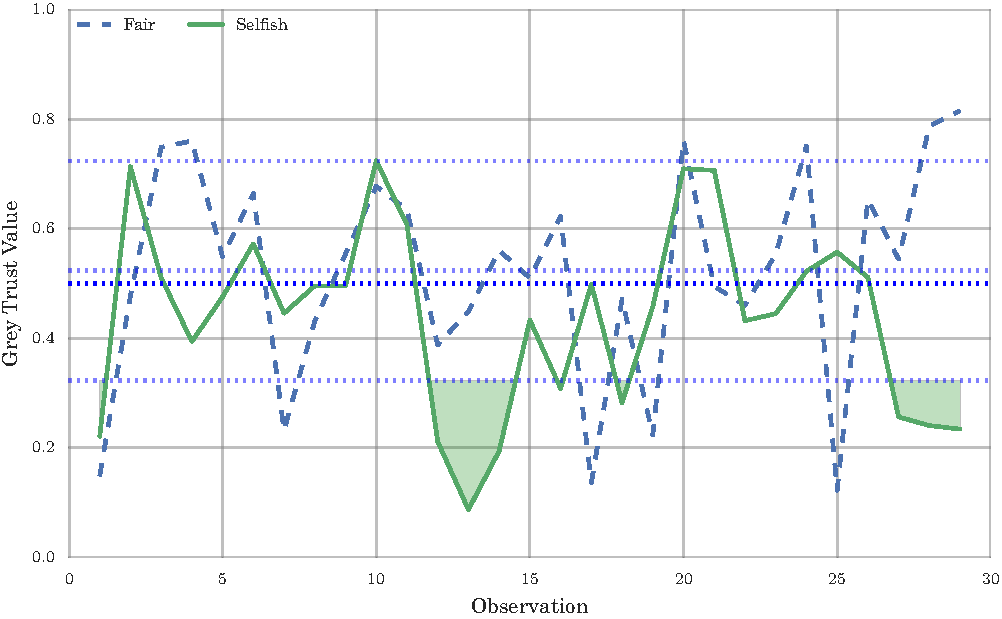
\includegraphics[width=.5\linewidth]{trust_bella_all_mobile_emph_RXThroughput_SelfishTargetSelection} \label{fig:all_mobile_selfish_rxthroughput}}
	\subfloat[TX Throughput]{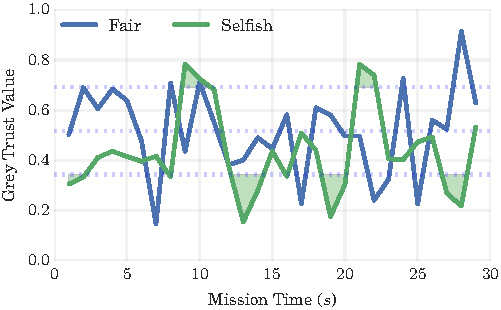
\includegraphics[width=.5\linewidth]{trust_bella_all_mobile_emph_TXThroughput_SelfishTargetSelection} \label{fig:all_mobile_selfish_txthroughput}}
	\caption{$T_{1,MTFM}$ in the All Mobile case for the STS behaviour, including dashed $\pm\sigma$ envelope about the fair scenario}
	\label{fig:all_mobile_selfish}
\end{figure}

\begin{figure}
	\centering
	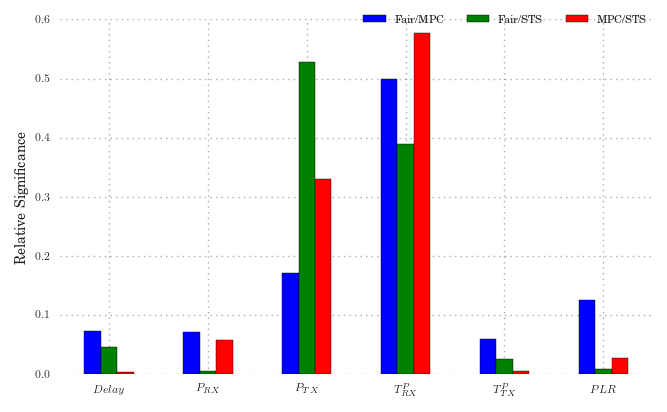
\includegraphics[width=0.65\linewidth]{MaliciousSelfishMetricFactors}
	\caption{Random Forest Factor Analysis of Malicious (MPC), Selfish (STS) and Fair behaviours compared against each-other}
	\label{fig:malselfactors}
\end{figure}

\begin{table}[h]
	\caption{Correlation Coefficients between metric weights and behaviour detection targets} \label{tab:correlations}
	\begin{center}
		\begin{tabular}{lcccccc}
			\toprule
			Correlation      & Delay & $P_{RX}$ & $P_{TX}$ & $T^P_{RX}$ & $T^P_{TX}$ & PLR \\
			\midrule
			Fair / MPC       & 0.199 &  0.159   & -0.416  &  0.708   & -0.238   & -0.401\\
			Fair / STS       & 0.179 &  -0.009  &  0.724  & -0.697   & -0.145   & -0.052\\
			MPC / STS        & 0.058 &  -0.134  &  0.146  & -0.768   &  0.052   &  0.146\\
			\bottomrule
		\end{tabular}
	\end{center}
\end{table}

\section{Changes to Assumptions}


Over the course of the  project, initial assumptions made about the nature, operation, and context of the project have changed wildly. This is largely due to the increased access to current and planned operational data from the Royal Navy while at DSTL Portsdown West, working with both the Naval Systems and Information Systems teams specifically on the area of maritime autonomy and the use of increasingly decentralised and autonomous systems for marine survey and observation. This work also contributed to a transnational collaboration looking at the establishment of systematic trust in autonomous systems.

Likewise, our work with Plextek and NPL on collaborative positioning using high precision timing was extremely helpful in developing my awareness not just of positioning techniques used by current platforms but also increased knowledge and time to generate simulation extensions to more accurately model not only the errors in these positioning systems but also algorithms for estimating the propagation time of acoustic comms.

\begingroup
\setlength{\LTleft}{-20cm plus -1fill}
\setlength{\LTright}{\LTleft}
\begin{longtable}{|p{0.3\textwidth}|p{0.8\textwidth}|}
	
	\hline \textbf{Initial Assumption} & \textbf{Correction} \\
	\endhead
	
	\hline AUV operation in open water &  AUVs (currently) mainly operate in coastal/littoral/riverbed areas with highly dynamic SSP (Speed of Sound Profile) and environmental variations.\newline
	Shallow environmental profile \\ 
	
	\hline  AUV sensing dynamically adjusts to the environment and motion &  SSS (Side Scanning Sonar) is extremely sensitive to not only height but strafe drift and can corrupt entire missions by being out of alignment more than 8-10m horizontally and 2-4m vertically (depending on initial configuration)\newline
	SAR (Synthetic Aperture Sonar), which builds up acoustic profiles over several ``pings'' is slightly more tolerant but any variation in path massively increases computational complexity of imagery (Possibly a ``Moore's Law'' Problem)\\ 
	
	\hline  AUV positioning is equally bad in all dimensions due to loss of GNSS, relying on INS, with cumulative errors on the order of tens of metres per hour of operation &  Depth sensing is extremely accurate\newline
	
	INS errors are directionally cumulative based on a electro/gyroscopic bias in the device. This means that if you travel two hours in one direction and two hours back in the opposite direction, your cumulative INS (Gyroscopic) error will be minimal\newline
	
	Additionally, the use of bottom tracking DVL (Doppler Velocity Log) provides quite good instantaneous velocity (through water) tracking but with normal errors. These errors are relative to the height above floor and cumulative with time.\newline
	
	All in all for most cases, drift can be characterised at around half the expected rate (~5/hr)\newline
	
	Simulation Model Characterisations have been generated for both Gyro and DVL error statistics\newline
	
	Further, collaborative measures can be taken to normalise these errors and consistently improve position accuracy by up to 40\%. This collaborative system has also been implemented into the simulation framework, and directly leads into the Scoundrel malicious behaviour model.\\ 
	
	\hline  --- Nodes operate with a spherical distribution (i.e. vertically and horizontally distributed) & All of these together lead to the the improved assumption that nodes operate in a flat arrangement, maintaining a known altitude for tracking accuracy, DVL consistency, SSS/SAR resolution and SSP stability. \\ 
	
	\hline  Acoustic Comms is terrible and curved &  This assumption was validated and expanded upon, with the generation of a simplified ``Bellhop'' simulation model generated to reasonably estimate the time of flight characteristics (but not ISI) of acoustic comms using ray tracing.\newline
	
	Current bitrates for $<$500m ranges are around the 100kbps scale, providing an upper limit on comms bandwidth for inter-node collaboration\\ 
	
	\hline  AUV operations will be mostly isolated &  Currently this is not the case, with AUV MHPC operations mainly based on either shore-based teams or Hunt/Sandown class based surface vessels in close proximity to operational area.\newline
	
	However BLOS (beyond line of sight) AUV operation is part of the MoD's Future Force 2020 programme so it is reasonable to continue operating as if that is the case.\\ 
	
	\hline  AUVs will be ``weaponless''&  While there are direct-disposal tethered ROVs fitted with explosive payloads, this assumption has largely borne out; the biggest blockade to having weaponised AUVs is legal trust in the security of operation of such an autonomous system, making it extremely unlikely that decentralised AUVs will ever be legally weaponised.\\ 
	
	\hline 
\end{longtable}
\endgroup

\section{Development, Publication Plans}

\subsection{Behaviour Detection}

Current work is concentrated on the improvement of the analysis of behaviours, with the intention of submission for publication of a paper on the threat detection methodology. This was intended to be completed last year but has fallen by the way-side in favour of the communications comparison work package.


\subsection{Multi-Domain Trust Assessment}

All remaining focus is on the cross domain implementation of trust, which is, combining communicative and behavioural trust assessments. 

This body of work has two main areas; analytical and critical. 

Initially, It is expected that this work will be largely analytical, maintaining context-free analysis for multi-domain trust but utilising AUV MANETs as an exemplar implementation for critical assessment of proposed cross-domain combination strategies.

This will require the completion of the implementation of existing communications TMF's for comparative assessment, including but not limited to Beta Expectation Values \cite{Li2007a}, Objective Trust Management Framework\cite{Li2008}, and Multi Parameter Trust Framework \cite{Guo11}

Ideally this work will go on as a Journal paper into potentially IEEE Comms, Dependable and Secure Computing, or Intelligent Systems Trans.

\subsection{Reactionary/Perturbative Trust}

It was hoped that some time be spent investigating reactionary behaviours, both communicative and physical, to allow a distributed, sparsely connected, decentralised team of nodes to dynamically ``interrogate'' or ``test'' the trustworthiness of nodes within the team. Given the compressed timeframe, this is unlikely.

\section{Proposed Thesis Chapter Titles}
\begin{enumerate} 
	\item Background Information on Trust and its applications to MANETs
	\begin{itemize}
		\item Discussion on abstract analysis of trust networks
		\item Discussion on the threat surface of Mobile Ad Hoc Networks and how that has been protected so far
		\item Introduction to Trust Management Frameworks and their benefits
	\end{itemize}
	\item Background Information on Maritime Uses of Autonomous Systems
	\begin{itemize}
		\item Discussion of current and future approaches to areas where autonomous systems can be used mainly focused on Mine counter measures, Hydrography and Patrol Capabilities (MHPC)
		\item Discussion of the contextual human factors around integrating autonomous systems into existing human-based solutions.
		\item Predominantly following on from work already accomplished under ``Analysis of Trust Interfaces in Autonomous and Semi-Autonomous Collaborative MHPC Operations'', including development of representative malicious and abnormal behaviours
	\end{itemize}
	\item Strategies for Multi-Domain Trust Assessment
	\begin{itemize}
		\item Analytical establishment of Multi-Domain Trust, from an information theoretic standpoint.
	\end{itemize}
	\item Modelling and Analysis of Collaborative Node Kinematic Behaviours in Underwater Acoustic MANETS
	\begin{itemize}
		\item Touching on the development of the simulation platform but focused on the mobility and assessment of mobility between nodes, including identification of suitable motive metrics and analyses of these motions to establish intent or abnormality
		\item Passing mention of work done in Drift analysis with NPL/Plextek as supporting evidence
	\end{itemize}
	\item Comparative Analysis of Multi-Domain Trust Assessment in Collaborative Mobile Networks
	\item Investigation into the relative performance characteristics of multi-domain combination strategies in an exemplary context (AUV teams) against existing single and multi metric TMFs
\end{enumerate}


\printbibliography
	
	
\end{document}